\chapter{实验结果及分析}
在前文中,本文针对跨域知识图谱中存在未见实体和未见关系的问题,提出了一个基于本体信息和元学习的知识表示学习模型。同时针对跨域知识表示学习中知识图谱语义信息的不足,本文提出了一种基于关系拓扑结构和描述文本的本体嵌入框架,通过获取本体信息并与图结构信息联合学习,实现了对未见实体和未见关系的特征聚合。结合元学习和本体嵌入技术,能够有效地处理跨域知识图谱中新实体和新关系的表示。为了验证模型的有效性,本章主要验证和评估了本文模型(NAMER)的实验效果。实验主要面向跨域情景的测试数据集进行,与现有的处理类似问题的归纳知识图谱表示模型进行对比。结果表明,引入了多层次的特征信息后,本文模型在实验数据上明显优于其他现有模型。最后的多个消融实验也证明了模型各个组成部分的重要性。

\section{数据集}
由于传统的知识图谱数据集通常基于“closed-world”设定,测试三元组中的实体和关系在训练数据集中已知,不存在跨域场景中的未见实体和未见关系。因此,为测试模型在包含未知实体和关系的跨域场景下的有效性,本文通过抽取包含本体层次三元组的DBpedia和NELL-995知识图谱的子集构建了新的数据集DB\_Ext和NELL\_Ext。

\subsection{源数据集介绍}
DBpedia:DBpedia是一个基于维基百科的语义知识库。该数据集由开源社区维护并使用维基百科文章和其他在线网络资源进行扩展。DBpedia从Wikipedia中提取结构化的数据,转化为事实三元组进行存储,包括图像、标签、描述文本等结构化属性,最新的数据集快照含有8.5亿条事实三元组数据。此外,DBpedia注重本体论的构建,本体类型数共768个,主要包括人物、地点、工作、组织等概念。这些实体、属性和关系通常以RDF图的形式存储,标准查询语言为SPARQL。DBpedia开源社区提供网页公布数据集的最新版本和统计数据,同时支持各数据集版本的检索和下载,为研究者使用提供了便利。

NELL-995:NELL-995数据集是根据NELL知识库抽取用于知识图谱补全任务的基准数据集。NELL (Never Ending Language Learning)是由卡内基梅隆大学领导的自动化学习系统,旨在从互联网的非结构化文本中自动提取知识。基于NELL知识库,NELL-995数据集包含995个实体和129个关系,覆盖地理、医学、体育、音乐、文化等广泛领域。NELL-995数据集的实体和关系被细粒度分类,每个实体被分配到一组多层次的关系类型中。因此,NELL-995数据集是学习细粒度知识表示和关系推理模型的理想数据集。

\subsection{任务数据集构建}
为了抽取出包含未见实体和关系的数据子集,本文首先构建一个包含所有三元组的实例知识图谱,在其中随机选取100个根实体节点并将每个节点的10个相邻接点组成测试子图,将子图中1/10的实体和关系标记为测试集,并从训练集中剔除这些实体和关系相关的三元组作为测试三元组;最终每个数据集中都包含了两个基本的子知识图谱,训练知识图谱\(\mathcal{G}^{train}\)和测试图谱\(\mathcal{G}^{test}\),后者包含了训练图谱中不存在的实体和关系。此外,为了测试模型对未见关系及未见实体的单独学习性能,在测试集中的query集设置中,本文将测试三元组分为三类:1、所有测试三元组中只包含了未见的实体(unseen\_ent);2、所有测试三元组中只包含了未见的关系(unseen\_rel);3、所有测试三元组中同时包含了未见的实体和关系(unseen\_both)。两个数据集中的统计数据如表\ref{tab:4-1}所示。其中,DB\_Ext数据集包含243个仅含未见实体的测试三元组、10个仅含未见关系的三元组和243个同时包含两个未见组件的三元组;NELL\_Ext数据集包含565个仅含未见实体的测试三元组、12个仅含未见关系的三元组和115个同时包含两个未见组件的三元组。各数据集包含三元组的统计数量如表\ref{tab:4-1}所示。
\begin{table}[h]
  \caption{数据集统计数据(括号中为未见组件数量)}
  \label{tab:4-1}
  \resizebox{\textwidth}{!}{%
  \begin{tabular}{@{}cccccccc@{}}
  \toprule
  {\color[HTML]{333333} }         & \multicolumn{3}{c}{{\color[HTML]{333333} 训练图谱}}                                                             & \multicolumn{4}{c}{{\color[HTML]{333333} 测试图谱}}                                                                                                                                                                                \\ \cmidrule(l){2-8} 
  {\color[HTML]{333333} }         & {\color[HTML]{333333} 实体数}  & {\color[HTML]{333333} 关系数} & {\color[HTML]{333333} 三元组数}                      & {\color[HTML]{333333} 实体数}      & {\color[HTML]{333333} 关系数}     & {\color[HTML]{333333} \begin{tabular}[c]{@{}c@{}}support\\ 三元组数\end{tabular}} & {\color[HTML]{333333} \begin{tabular}[c]{@{}c@{}}query\\ 三元组数\end{tabular}} \\ \midrule
  {\color[HTML]{333333} NELL\_Ext} & {\color[HTML]{333333} 1583} & {\color[HTML]{333333} 153} & \multicolumn{1}{c|}{{\color[HTML]{333333} 5269}} & {\color[HTML]{333333} 851(753)} & {\color[HTML]{333333} 140(30)} & {\color[HTML]{333333} 2160}                                                   & {\color[HTML]{333333} 692}                                                  \\
  {\color[HTML]{333333} DB\_Ext}   & {\color[HTML]{333333} 795}  & {\color[HTML]{333333} 115} & \multicolumn{1}{c|}{{\color[HTML]{333333} 1508}} & {\color[HTML]{333333} 913(884)} & {\color[HTML]{333333} 128(46)} & {\color[HTML]{333333} 1930}                                                   & {\color[HTML]{333333} 496}                                                  \\ \bottomrule
  \end{tabular}%
  }
  \end{table}
% \begin{table}[h]
%   \caption{数据集统计数据(括号中为未见组件数量)}
%   \label{tab:4-1}
%   \resizebox{\textwidth}{!}{%
%   \begin{tabular}{cccccccc}
%   \hline
%                       & \multicolumn{3}{c}{训练图谱}                                                                                    & \multicolumn{4}{c}{测试图谱}                                                                                                                                                         \\ \cline{2-8} 
%   \multirow{-2}{*}{} & 实体数                         & 关系数                        & 三元组数                                             & 实体数                             & 关系数                            & \begin{tabular}[c]{@{}c@{}}support\\ 三元组数\end{tabular} & \begin{tabular}[c]{@{}c@{}}query\\ 三元组数\end{tabular} \\ \hline
%   NELL\_Ext          & {\color[HTML]{333333} 1583} & {\color[HTML]{333333} 153} & \multicolumn{1}{c|}{{\color[HTML]{333333} 5269}} & {\color[HTML]{333333} 851(753)} & {\color[HTML]{333333} 140(30)} & {\color[HTML]{333333} 2160}                            & {\color[HTML]{333333} 692}                           \\
%   DB\_Ext            & {\color[HTML]{333333} 795}  & {\color[HTML]{333333} 115} & \multicolumn{1}{c|}{{\color[HTML]{333333} 1508}} & {\color[HTML]{333333} 913(884)} & {\color[HTML]{333333} 128(46)} & {\color[HTML]{333333} 1930}                            & {\color[HTML]{333333} 496}                           \\ \hline
%   \end{tabular}%
%   }
%   \end{table}

\section{模型参数设置}
对于用于对比的基准模型,本文采用了相关论文给出的最优超参数设置,本文模型采用的相关参数设置如表\ref{tab:4-2}所示。
% \begin{table}[h]
%   \caption{模型超参数设置}
%   \label{tab:4-2}
%   \resizebox{\textwidth}{!}{%
%   \begin{tabular}{cc|cc|cc}
%   \hline
%   {\color[HTML]{333333} 本体嵌入参数}          & {\color[HTML]{333333} 设置值}     & {\color[HTML]{333333} 元学习训练参数}             & {\color[HTML]{333333} 设置值}    & {\color[HTML]{333333} 嵌入参数}       & {\color[HTML]{333333} 设置值} \\ \hline
%   {\color[HTML]{333333} lr}              & {\color[HTML]{333333} 0.00005} & {\color[HTML]{333333} lr}                  & {\color[HTML]{333333} 0.001}  & {\color[HTML]{333333} dim}        & {\color[HTML]{333333} 300} \\
%   {\color[HTML]{333333} ent\_str\_dim}     & {\color[HTML]{333333} 150}     & {\color[HTML]{333333} train\_bs}            & {\color[HTML]{333333} 64}     & {\color[HTML]{333333} num\_gcn}    & {\color[HTML]{333333} 2}   \\
%   {\color[HTML]{333333} ent\_text\_dim}    & {\color[HTML]{333333} 300}     & {\color[HTML]{333333} eval\_bs}             & {\color[HTML]{333333} 16}     & {\color[HTML]{333333} num\_comgcn} & {\color[HTML]{333333} 2}   \\
%   {\color[HTML]{333333} mapping\_size}    & {\color[HTML]{333333} 300}     & {\color[HTML]{333333} num\_step}            & {\color[HTML]{333333} 100000} & {\color[HTML]{333333} gcn\_dim}    & {\color[HTML]{333333} 300} \\
%   {\color[HTML]{333333} training\_epochs} & {\color[HTML]{333333} 1000}    & {\color[HTML]{333333} early\_stop\_patience} & {\color[HTML]{333333} 20}     & {\color[HTML]{333333} hid\_drop}   & {\color[HTML]{333333} 0.3} \\
%   {\color[HTML]{333333} batch\_size}      & {\color[HTML]{333333} 100}     & {\color[HTML]{333333} num\_sample\_size}     & {\color[HTML]{333333} 10}     & {\color[HTML]{333333} -}          & {\color[HTML]{333333} -}   \\ \hline
%   \end{tabular}%
%   }
%   \end{table}
% \begin{table}[h]
%   \caption{模型超参数设置}
%   \label{tab:4-2}
%   \resizebox{\textwidth}{!}{%
%   \begin{tabular}{|c|c|c|c|c|c|}
%   \hline
%   {\color[HTML]{333333} 本体嵌入参数}           & {\color[HTML]{333333} 设置值}     & {\color[HTML]{333333} 元学习训练参数}                          & {\color[HTML]{333333} 设置值}    & {\color[HTML]{333333} 嵌入参数}        & {\color[HTML]{333333} 元学习训练参数} \\ \hline
%   {\color[HTML]{333333} lr}               & {\color[HTML]{333333} 0.00005} & {\color[HTML]{333333} lr}                               & {\color[HTML]{333333} 0.001}  & {\color[HTML]{333333} dim}         & {\color[HTML]{333333} 300}     \\ \hline
%   {\color[HTML]{333333} ent\_str\_dim}    & {\color[HTML]{333333} 150}     & {\color[HTML]{333333} train\_bs}                        & {\color[HTML]{333333} 64}     & {\color[HTML]{333333} num\_gcn}    & {\color[HTML]{333333} 2}       \\ \hline
%   {\color[HTML]{333333} ent\_text\_dim}   & {\color[HTML]{333333} 300}     & {\color[HTML]{333333} eval\_bs}                         & {\color[HTML]{333333} 16}     & {\color[HTML]{333333} num\_comgcn} & {\color[HTML]{333333} 2}       \\ \hline
%   {\color[HTML]{333333} mapping\_size}    & {\color[HTML]{333333} 300}     & {\color[HTML]{333333} num\_step}                        & {\color[HTML]{333333} 100000} & {\color[HTML]{333333} gcn\_dim}    & {\color[HTML]{333333} 300}     \\ \hline
%   {\color[HTML]{333333} training\_epochs} & {\color[HTML]{333333} 1000}    & {\color[HTML]{333333} early\_stop\_patience}            & {\color[HTML]{333333} 20}     & {\color[HTML]{333333} hid\_drop}   & {\color[HTML]{333333} 0.3}     \\ \hline
%   {\color[HTML]{333333} batch\_size}      & {\color[HTML]{333333} 100}     & {\color[HTML]{333333} num\_sample\_for\_estimate\_size} & {\color[HTML]{333333} 10}     & {\color[HTML]{333333} -}           & {\color[HTML]{333333} -}       \\ \hline
%   \end{tabular}%
%   }
% \end{table}

其中主要包含以下三个方面的参数设置:
\begin{enumerate}[label=\arabic*)]
\item 本体嵌入相关参数:模型学习率lr、本体三元组概念节点结构嵌入维度ent\_str\_dim、本体概念节点文本嵌入维度ent\_text\_dim、线性隐藏层维度mapping\_size以及训练的epoch数量和batch的大小。
\item 元学习相关参数:任务学习率lr、单任务支持集的batch数量train\_bs、单任务查询集的batch数量eval\_bs、元训练总任务数num\_step、元训练提前结束无效训练任务计数early\_stop\_patience以及单个batch采样的根节点数。
\item 图谱嵌入相关参数:基本维度的设置dim、关系位置图对关系进行GCN的层数num\_gcn、GCN中间传递维度gcn\_dim以及GCN层的丢弃率hid\_drop、对关系和实体进行联合学习的CompGCN的层数。
\end{enumerate}
\begin{table}[h]
  \caption{模型超参数设置}
  \label{tab:4-2}
  \resizebox{\textwidth}{!}{%
  \begin{tabular}{@{}cccccc@{}}
  \toprule
  {\color[HTML]{333333} \textbf{本体嵌入参数}} & {\color[HTML]{333333} \textbf{设置值}}                 & {\color[HTML]{333333} \textbf{元学习训练参数}}    & {\color[HTML]{333333} \textbf{设置值}}                & {\color[HTML]{333333} \textbf{嵌入参数}} & {\color[HTML]{333333} \textbf{设置值}} \\ \midrule
  {\color[HTML]{333333} lr}              & \multicolumn{1}{c|}{{\color[HTML]{333333} 0.00005}} & {\color[HTML]{333333} lr}                  & \multicolumn{1}{c|}{{\color[HTML]{333333} 0.001}}  & {\color[HTML]{333333} dim}           & {\color[HTML]{333333} 300}          \\
  {\color[HTML]{333333} ent\_str\_dim}     & \multicolumn{1}{c|}{{\color[HTML]{333333} 150}}     & {\color[HTML]{333333} train\_bs}            & \multicolumn{1}{c|}{{\color[HTML]{333333} 64}}     & {\color[HTML]{333333} num\_gcn}       & {\color[HTML]{333333} 2}            \\
  {\color[HTML]{333333} ent\_text\_dim}    & \multicolumn{1}{c|}{{\color[HTML]{333333} 300}}     & {\color[HTML]{333333} eval\_bs}             & \multicolumn{1}{c|}{{\color[HTML]{333333} 16}}     & {\color[HTML]{333333} num\_comgcn}    & {\color[HTML]{333333} 2}            \\
  {\color[HTML]{333333} mapping\_size}    & \multicolumn{1}{c|}{{\color[HTML]{333333} 300}}     & {\color[HTML]{333333} num\_step}            & \multicolumn{1}{c|}{{\color[HTML]{333333} 100000}} & {\color[HTML]{333333} gcn\_dim}       & {\color[HTML]{333333} 300}          \\
  {\color[HTML]{333333} training\_epochs} & \multicolumn{1}{c|}{{\color[HTML]{333333} 1000}}    & {\color[HTML]{333333} early\_stop\_patience} & \multicolumn{1}{c|}{{\color[HTML]{333333} 20}}     & {\color[HTML]{333333} hid\_drop}      & {\color[HTML]{333333} 0.3}          \\
  {\color[HTML]{333333} batch\_size}      & \multicolumn{1}{c|}{{\color[HTML]{333333} 100}}     & {\color[HTML]{333333} num\_sample\_size}     & \multicolumn{1}{c|}{{\color[HTML]{333333} 10}}     & {\color[HTML]{333333} -}             & {\color[HTML]{333333} -}            \\ \bottomrule
  \end{tabular}%
  }
  \end{table}

在对三元组进行打分评估时,本文通过对CompGCN第二层输出的改进,可支持多种KGE模型作为评分函数。实际采用的KGE模型包含TransE、DistMult、ComplEx及RotatE。实体和关系的维度根据采用的KGE模型在基础嵌入维度上进行调整,具体如下表\ref{tab:4-3}所示:
\begin{table}[h]
  \caption{评分函数}
  \label{tab:4-3}
  \centering
  \resizebox{0.6\textwidth}{!}{%
  \begin{tabular}{@{}cccc@{}}
  \toprule
  {\color[HTML]{333333} \textbf{模型名}} & {\color[HTML]{333333} \textbf{实体维度}} & {\color[HTML]{333333} \textbf{关系维度}} & {\color[HTML]{333333} \textbf{评分函数}}        \\ \midrule
  {\color[HTML]{333333} TranE}        & {\color[HTML]{333333} dim}           & {\color[HTML]{333333} dim}           & {\color[HTML]{333333} F = -|| h + r - t ||} \\
  {\color[HTML]{333333} DistMult}     & {\color[HTML]{333333} dim}           & {\color[HTML]{333333} dim}           & {\color[HTML]{333333} F = \(\rm h^{T}\) diag(r) t}     \\
  {\color[HTML]{333333} ComplEx}      & {\color[HTML]{333333} 2 * dim}       & {\color[HTML]{333333} 2 * dim}       & {\color[HTML]{333333} F = Re(\(\rm h^{T}\) diag(r) t)} \\
  {\color[HTML]{333333} RotatE}       & {\color[HTML]{333333} 2 * dim}       & {\color[HTML]{333333} dim}           & {\color[HTML]{333333} F = -|| h ○ r - t ||} \\ \bottomrule
  \end{tabular}%
  }
  \end{table}
% \begin{table}[h]
%   \caption{评分函数}
%   \label{tab:4-3}
%   \centering
%   \resizebox{0.7\textwidth}{!}{%
%   \begin{tabular}{cccc}
%   \hline
%   {\color[HTML]{333333} 模型名}      & {\color[HTML]{333333} 实体维度}    & {\color[HTML]{333333} 关系维度}    & {\color[HTML]{333333} 评分函数}                 \\ \hline
%   {\color[HTML]{333333} TranE}    & {\color[HTML]{333333} dim}     & {\color[HTML]{333333} dim}     & {\color[HTML]{333333} F = -|| h + r - t ||} \\
%   {\color[HTML]{333333} DistMult} & {\color[HTML]{333333} dim}     & {\color[HTML]{333333} dim}     & {\color[HTML]{333333} F = \(\rm h^{T}\) diag(r) t}     \\
%   {\color[HTML]{333333} ComplEx}  & {\color[HTML]{333333} 2 * dim} & {\color[HTML]{333333} 2 * dim} & {\color[HTML]{333333} F = Re(\(\rm h^{T}\) diag(r) t)} \\
%   {\color[HTML]{333333} RotatE}   & {\color[HTML]{333333} 2 * dim} & {\color[HTML]{333333} dim}     & {\color[HTML]{333333} F = -|| h ○ r - t ||} \\ \hline
%   \end{tabular}%
%   }
%   \end{table}
% \begin{table}[h]
%   \caption{评分函数}
%   \label{tab:4-3}
%   \centering
%   \resizebox{0.8\textwidth}{!}{%
%   \begin{tabular}{|l|l|l|l|}
%   \hline
%   {\color[HTML]{333333} 模型名}      & {\color[HTML]{333333} 实体维度}    & {\color[HTML]{333333} 关系维度}    & {\color[HTML]{333333} 评分函数}                 \\ \hline
%   {\color[HTML]{333333} TranE}    & {\color[HTML]{333333} dim}     & {\color[HTML]{333333} dim}     & {\color[HTML]{333333} F = -|| h + r - t ||} \\ \hline
%   {\color[HTML]{333333} DistMult} & {\color[HTML]{333333} dim}     & {\color[HTML]{333333} dim}     & {\color[HTML]{333333} F = \(\rm h^{T}\) diag(r) t}     \\ \hline
%   {\color[HTML]{333333} ComplEx}  & {\color[HTML]{333333} 2 * dim} & {\color[HTML]{333333} 2 * dim} & {\color[HTML]{333333} F = Re(\(\rm h^{T}\) diag(r) t)} \\ \hline
%   {\color[HTML]{333333} RotatE}   & {\color[HTML]{333333} 2 * dim} & {\color[HTML]{333333} dim}     & {\color[HTML]{333333} F = -|| h ○ r - t ||} \\ \hline
%   \end{tabular}%
%   }
% \end{table}

其中评分函数中的h、r、t分别指代头实体、关系和尾实体的嵌入表示,Re表示复向量的实部分量,○操作表示旋转操作。

\section{实验设计及评价指标}
本实验包含本体嵌入表示学习和图谱表示学习两个阶段,第一个阶段主要学习到融合描述文本信息的本体嵌入表示,第二阶段使用本体信息进行跨域知识图谱的表示学习。

第一阶段首先采用传统的表示学习方法对本体三元组数据进行初步嵌入表示。其次,从预训练词嵌入glove中获取本体描述信息中各描述单词的初始化词向量。使用TF-IDF统计方法识别单词的重要程度,并对单词的词向量进行加权聚合计算,以获得本体节点描述文本的初始化向量嵌入。最后,将本体三元组的结构化表示嵌入和本体描述文本的表示嵌入映射到同一个空间,以进行评分和更新,从而获得拼接后的最终本体嵌入。

第二阶段对跨域知识图谱进行表示学习,为了在元学习中模拟出跨域场景,在每个元学习任务的设置中都人为抹除了一些实体和关系的标签,使得这些实体和关系必须通过本文模型的未见关系和未见实体嵌入模块学习得到向量表示,而不是从传统嵌入方法的嵌入矩阵中取得。

对于模型在链接预测任务上的评价指标,本文选取了MRR和Hit@10作为评判的标准。其中MRR通过预测三元组排名的倒数来进行计算,即对测试三元组中的所有事实三元组,如果该三元组在预测排名靠前,对应的倒数也会比较大,因此链接预测性能与MRR评价指标的数值大小成正相关。而Hits@n描述的是在所有预测三元组排名中前n的三元组所占的平均比例,其计算公式如公式\ref{eq:5-1}所示:
\begin{equation}
  HITS@n = \frac{1}{|S|} \sum_{i=1}^{|S|}||(rank_{i} \leqslant n) \label{eq:5-1}
\end{equation}

假设n设置为10,那么统计事实三元组在预测三元组中前n名的个数,最后再除以总个数就得到了Hits@10的结果,其中\(||(·)\)为indicator函数(若条件真则函数值为1,否则为0)。

参与比较的模型如下:

Neural-LP\cite{yang2017differentiable}(2017):该模型基于知识库构建了一个可学习逻辑规则的可微模型。逻辑规则是独立于实体和关系的,因此理论上该模型可在任何未见的实体上应用,并在归纳图谱补全任务中相比传统方法(即对实体进行结构信息表示学习)有明显提升。

DURM\cite{sadeghian2019drum}(2019):提出了一种可微的、可同时学习规则逻辑及其置信度得分的方法。该方法可以使用梯度优化来处理归纳逻辑编程任务,并可用于处理含有未知实体的链接预测任务。

GraIL\cite{teru2020inductive}(2020):该模型不直接学习实体节点嵌入,也没有使用任何节点的属性。相反,它在测试三元组候选关系的周围构建子图,并利用子图的结构和结构化的节点特征来预测三元组。这使得该模型能够很好地应用于未知的实体三元组预测任务。

CoMPILE\cite{mai2021communicative}(2021):该模型对GraIL模型子图归纳模型进行了改进,包括加强对子图关系方向性的限制,并在未知节点特征聚合的信息传递过程中增加了先前模型中忽略的关系特征。

MaKEr\cite{chen2019meta}(2022):该模型通过学习关系结构的特征来聚合邻接关系的特征,进而对关系进行表示,并聚合关系特征对实体进行编码。模型利用拓扑结构的信息,在一定程度上实现对未见实体和未见关系的表示。

\section{实验结果及分析}
各模型在NELL\_Ext上的链接预测任务实验结果如下表\ref{tab:4-4}所示,各模型在DB\_Ext上的链接预测任务实验结果如表\ref{tab:4-5}所示。根据测试数据集的三元组对未知实体和关系的包含情况,将结果分为了只包含未见实体的结果(u\_ent)、只包含未见关系的结果(u\_rel)以及同时包含未见实体和未见关系的结果(u\_both)。表格中加粗部分为最优的实验效果,带有下划线的则是该类基准模型中表现最优的得分,模型括号中指代的是在评分阶段采用的KGE评分函数。
\begin{table}[h]
  \caption{NELL\_Ext数据集结果}
  \label{tab:4-4}
  \resizebox{\textwidth}{!}{%
  \begin{tabular}{ccccccc}
  \hline
  \multicolumn{7}{c}{NELL\_Ext}                                                                                                                 \\ \hline
 {\multirow{2}{*}{}} & \multicolumn{2}{c}{u\_ent}       & \multicolumn{2}{c}{u\_rel}       & \multicolumn{2}{c}{u\_both}      \\ \cline{2-7} 
               & MRR            & Hits@10        & MRR            & Hits@10        & MRR            & Hits@10        \\ \hline
  \multicolumn{1}{c|}{Neural-LP}         & 30.48          & 47.96          & -              & -              & -              & -              \\
  \multicolumn{1}{c|}{DRUM}              & 31.82          & 48.32          & -              & -              & -              & -              \\
  \multicolumn{1}{c|}{GraIL}             & 71.62          & 92.92          & -              & -              & -              & -              \\
  \multicolumn{1}{c|}{CoMPILE}           & {\ul 75.94}    & {\ul 93.62}    & -              & -              & -              & -              \\ \hline
  \multicolumn{1}{c|}{MaKEr(TransE)}     & 70.82          & 92.00          & 24.56          & 54.17          & 21.53          & 51.74          \\
  \multicolumn{1}{c|}{MaKEr(DistMult)}   & 70.63          & 91.33          & 27.02          & 60.00          & \textbf{41.39} & 57.65          \\
  \multicolumn{1}{c|}{MaKEr(ComplEx)}    & 72.24          & 91.91          & 18.27          & 34.17          & 29.39          & 59.65          \\
  \multicolumn{1}{c|}{MaKEr(RotatE)}     & {\ul 77.09}    & {\ul 94.64}    & {\ul 31.53}    & {\ul 55.00}    & 31.45          & {\ul 62.35}    \\ \hline
  \multicolumn{1}{c|}{NAMER(TransE)}     & 78.28          & 94.86          & 20.72          & 53.34          & 27.11          & 55.85          \\
  \multicolumn{1}{c|}{NAMER(DistMult)}   & 75.98          & 92.46          & 19.30          & 22.50          & 31.37          & 55.65          \\
  \multicolumn{1}{c|}{NAMER(ComplEx)}    & 73.61          & 90.60          & 24.44          & 38.33          & 29.70          & 54.96          \\
  \multicolumn{1}{c|}{NAMER(RotatE)}     & \textbf{79.92} & \textbf{94.73} & \textbf{45.07} & \textbf{75.63} & {\ul 40.33}    & \textbf{67.06} \\ \hline
  \end{tabular}%
  }
  \end{table}
\begin{table}[h]
  \caption{DB\_Ext数据集结果}
  \label{tab:4-5}
  \resizebox{\textwidth}{!}{%
  \begin{tabular}{ccccccc}
  \hline
  \multicolumn{7}{c}{DB\_Ext}                                                                                                                 \\ \hline
                 & \multicolumn{2}{c}{u\_ent}       & \multicolumn{2}{c}{u\_rel}       & \multicolumn{2}{c}{u\_both}      \\ \cline{2-7} 
               & MRR            & Hits@10        & MRR            & Hits@10        & MRR            & Hits@10        \\ \hline
  \multicolumn{1}{c|}{Neural-LP}       & 57.15          & 73.46          & -              & -              & -              & -              \\
  \multicolumn{1}{c|}{DRUM}            & 59.88          & 73.25          & -              & -              & -              & -              \\
  \multicolumn{1}{c|}{GraIL}           & 59.44          & {\ul 80.86}    & -              & -              & -              & -              \\
  \multicolumn{1}{c|}{CoMPILE}         & {\ul 60.66}    & 79.93          & -              & -              & -              & -              \\ \hline
  \multicolumn{1}{c|}{MaKEr(TransE)}   & 54.4           & 83.7           & 31.13          & 54.00          & 38.66          & 66.5           \\
  \multicolumn{1}{c|}{MaKEr(DistMult)} & 46.24          & 81.07          & 16.43          & 11.00          & 32.16          & 56.71          \\
  \multicolumn{1}{c|}{MaKEr(ComplEx)}  & 53.79          & 82.47          & 19.95          & 29.00          & 36.88          & 59.26          \\
  \multicolumn{1}{c|}{MaKEr(RotatE)}   & {\ul 59.55}    & {\ul 86.09}    & {\ul 32.93}    & {\ul 55.00}    & \textbf{41.27} & {\ul 66.54}    \\ \hline
  \multicolumn{1}{c|}{NAMER(TransE)}   & 64.63          & 89.60          & \textbf{44.77} & 70.25          & 34.92          & \textbf{69.42} \\
  \multicolumn{1}{c|}{NAMER(DistMult)} & 56.73          & 80.25          & 13.68          & 11.00          & 33.94          & 61.74          \\
  \multicolumn{1}{c|}{NAMER(ComplEx)}  & 52.22          & 77.34          & 14.40          & 15.00          & 31.72          & 59.49          \\
  \multicolumn{1}{c|}{NAMER(RotatE)}   & \textbf{66.43} & \textbf{89.67} & 41.80          & \textbf{74.00} & {\ul 35.11}    & 63.81          \\ \hline
  \end{tabular}%
  }
\end{table}

表\ref{tab:4-4}和表\ref{tab:4-5}展示了各模型在NELL\_Ext和DB\_Ext上的链接预测结果。计算Hit@10分数时,本文选取了50个候选进行评估,并对于不同的补全任务(u\_ent、u\_rel和u\_both)显示了不同模型的得分。GraIL、Neural-LP、DRUM和CoMPILE仅针对未见实体补全任务设计了实验,因此未列出其在未见关系上的实验结果。上述数据均为模型运行4次后取平均值的结果。

结果表明,本文提出的NAMER模型相比其他基准模型有所改进,并在不同的KGE评分模型上有不同程度的提升。此外,基于RotatE的NAMER模型总体取得了最好的成绩。我们认为RotatE模型采用了更加复杂的关系和实体的映射关系,因此能表现更多没有重叠的特征信息。这也证明了本文模型的有效性。

本文在处理未见实体的测试集上,首先比较了依据规则学习来处理未见实体的Neural-LP模型和DRUM模型以及基于子图推理的GraIL模型和CoMPILE模型。结果表明,基于规则的模型的效果不如基于子图的模型,在 NELL\_Ext 数据集上,Neural-LP和DRUM的实验得分远低于GraIL和CoMPILE模型。这是由于基于规则的模型依赖于针对数据集学习出的规则,需要大量的数据集或对样本均衡性有严格的要求,因此模型效果受数据集影响较大。CoMPILE模型在GraIL模型的基础上强调了关系的重要性,总体效果要比GraIL表现更好。然而,上述四个模型都无法处理未见关系,而基于子图归纳推理的模型强调测试三元组中头尾实体间的局部子图信息,没有完全利用到实体周围的结构特征信息以及关系信息,整体效果都比本文的模型差。比较本文的模型与MaKEr模型,MaKEr模型在MRR的评价指标上平均低了4.42\%,而在对应RotatE评分函数下的Hits@10评价指标上,本文模型表现领先了1.85\%。尽管MaKEr模型考虑到了关系对实体的重要性,但在关系表示的特征学习方面,没有充分利用图谱的语义知识,所以效果比本文模型差。这进一步说明了本文模型在未见实体表示方面的有效性。

本文在仅包含未见关系和同时包含未见实体和关系的测试集上,与通过结构信息对关系和实体进行编码的MaKEr模型进行了比较。针对未知关系,本文引入了额外的本体知识作为关系语义信息的补充,并利用关系图卷积对关系的表示进行了更新,以学习未见关系周围的结构拓扑信息。两个测试集上的实验结果表明,相比于仅使用结构信息编码关系的MaKEr模型,本文引入本体信息能够有效补充关系表示的语义信息。在处理未知关系时,本文采用RotatE作为评分函数的模型表现出明显的优势,在NELL\_Ext数据集上的MRR得分比MaKEr高出14.54\%,而在Hits@10的得分方面,70.63的得分比MaKEr的得分高出约20\%。这表明本文模型在捕捉关系语义和结构信息方面具有更好的性能,在考虑局部关系和全局关系时都表现良好。在同时包含两种未知组件的测试集上,本文模型相比MaKEr模型在NELL\_Ext数据集的Hits@10评分上平均提升了1.82\%,在DB\_Ext数据集的MRR和Hits@10分别平均提升了1.18\%和0.53\%。

此外,本文实验发现,相比于DistMult和ComplEx模型,将TransE和RotatE用作解码器时模型效果更好,尤其在处理关系方面。在本体嵌入实验中,本文采用RotatE作为评分函数来对本体信息进行表示学习。DistMult和ComplEx模型因其复杂性与RotatE的本体嵌入方法不兼容而效果下降。相比之下,TransE模型简单易操作,在进行特征提取时更为适合。与本文模型搭配整体表现最好的RotatE模型不仅与本体嵌入方法相匹配,还能够提供更全面的对实体和关系低维度嵌入表示,因此在本文中表现为最优的模型之一。

\section{模型消融实验}
本节将介绍模型中几个重要模块的多项消融实验,以展示本文模型各部分的重要性,主要设置了5项不同的消融设置实验:(1)去除元学习的设置;(2)去除本体的设置;(3)去除实体聚合表示的设置;(4)去除关系GCN聚合的设置;(5)同时去除本体和元学习的设置。获得的实验结果如表\ref{tab:4-6}所示:
\begin{table}[h]
  \caption{在NELL\_Ext上的消融实验结果}
  \resizebox{\textwidth}{!}{%
  \label{tab:4-6}
  \begin{tabular}{ccccccc}
  \hline
  \multicolumn{7}{c}{NELL\_Ext}                                                                                                                  \\ \hline
                    & \multicolumn{2}{c}{u\_ent}       & \multicolumn{2}{c}{u\_rel}       & \multicolumn{2}{c}{u\_both}      \\ \cline{2-7} 
                 & MRR            & Hits@10        & MRR            & Hits@10        & MRR            & Hits@10        \\ \hline
  \multicolumn{1}{c|}{NAMER(TransE)}      & \textbf{78.28} & \textbf{94.86} & 20.72          & 53.34          & \textbf{27.11} & \textbf{55.85} \\ \hline
  \multicolumn{1}{c|}{no\_meta\_TransE}     & 29.31          & 43.82          & 12.65          & 30.83          & 10.18          & 22.26          \\
  \multicolumn{1}{c|}{no\_ont\_TransE}      & 76.89          & 94.07          & 14.96          & 27.50          & 14.06          & 28.78          \\
  \multicolumn{1}{c|}{no\_ent\_TransE}      & 76.85          & 94.07          & 18.00          & 55.83          & 19.43          & 50.7           \\
  \multicolumn{1}{c|}{no\_gcn\_TransE}      & 74.68          & 92.27          & \textbf{23.88} & \textbf{61.67} & 19.85          & 46.26          \\
  \multicolumn{1}{c|}{no\_meta\_ont\_TransE} & 26.57          & 38.69          & 11.15          & 25.00          & 12.62          & 27.74          \\ \hline
  \end{tabular}%
  }
  \end{table}

其中每个消融实验的具体设置如下:
\begin{enumerate}[label=\arabic*)]
  \item 去除元学习的设置:在模型训练阶段,本文引入了元学习,在训练集上提取任务子图并通过随机标签来模拟出未见的组件从而训练出模型处理未见组件的能力。在该消融实验下,取消掉了对子图标签的模拟效果即按照传统KGE模型的训练方法,在训练集上对所有三元组进行嵌入和损失计算。
  \item 去除本体的设置:本文模型的一个创新点即在对关系嵌入表示的时候通过关系位置图加入本体信息进行学习,在该消融实验设置下,将本体信息替换为随机表示对未见关系进行特征学习。
  \item 去除实体聚合表示的设置:本文模型在处理未见实体时,采用该实体周围的关系信息聚合表示,在该消融实验设置下对未见实体进行随机化嵌入设置,考察未见实体的表示模块。
  \item 去除关系GCN聚合的设置:在构建完关系的位置图并引入本体嵌入后,本文模型通过GCN来加强关系对邻接结构的特征学习,该消融实验下去除两层GCN层,直接使用本体信息。
  \item 同时去除本体和元学习设置:同时结合消融实验(1)和(2)的设置。
\end{enumerate}

将消融实验结果与NAMER(TransE)模型在NELL\_Ext上的实验结果进行比较,可以看出,基本所有的消融设置都会导致性能下降,表明上述各模块的重要性。但是在去除关系GCN聚合的设置上,在仅含有未见关系的测试集上效果反而提升,分析可知该层GCN的作用是在关系本体嵌入的基础上学习关系邻接关系的结构信息。这些结构信息的引入一定程度上会影响仅对关系的表示效果,导致在仅包含未见关系的测试集上的效果下降。但是这些结构信息的引入在未见实体的表示中,因为实体需要聚合邻接关系进行表示,因此引入的结构信息会对实体的表示效果进行提升,可以发现去掉GCN在包含未见实体和同时包含未见实体和未见关系的测试集上效果都有明显的下降,因此也侧面证明了GCN模型对实验效果提升的必要性。此外,本文观察到元学习设置对模型性能至关重要,表明在推广到测试知识图谱的任务上对模型进行元训练的有效性。

\section{未见实体案例分析}
\begin{figure}[h]
  \centering
  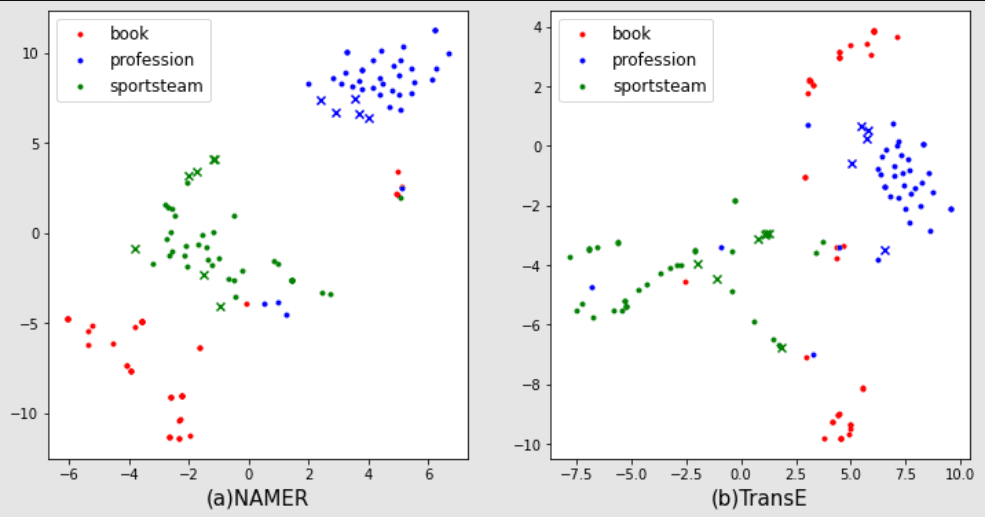
\includegraphics[width=0.75\textwidth]{4-1.png}
  \caption{实体嵌入可视化分析}
  \label{fig:4-1}
\end{figure}
图\ref{fig:4-1}中展示了本文提出的NAMER模型和去除元学习和本体嵌入的传统TransE模型在NELL-Ext数据集的测试集上实体嵌入的可视化。图中不同颜色展示了不同类型的实体,圆点代表未见的实体,叉号则代表了该类型下的已知实体。NAMER在实体获得初始化的向量表示后,通过两层GCN来学习邻域节点和相连关系的特征,使得同一类型的实体在表示空间上尽可能聚集在较紧密的邻域中。从可视化中也可以看出NAMER产生的嵌入分布与对应类型更加一致,在嵌入映射的距离上更近紧凑,而TransE-KGE产生的嵌入则混合了不同实体类型。NAMER将嵌入映射到了不同的聚类中,而TransE中不同实体类型的嵌入则混合在一起。此外,本文的模型在对未见的实体进行表示学习的过程中,采用聚合实体关系的特征来初始化实体向量,相邻关系的结构特征可以表现出实体的类型信息,因此模型可以将未见的实体的嵌入与同一类型的已知实体聚类。不同类型实体的聚类表明,NAMER能够用包含合理语义和信息性知识的嵌入来表示未见的实体。

\section{未见关系案例分析}
对于未见关系,本文同样选取了部分关系映射到了二维空间上进行可视化分析,如图\ref{fig:4-2}所示,其中圆点代表训练集中可见的关系,叉号代表测试集中的未见关系。
\begin{figure}[h]
  \centering
  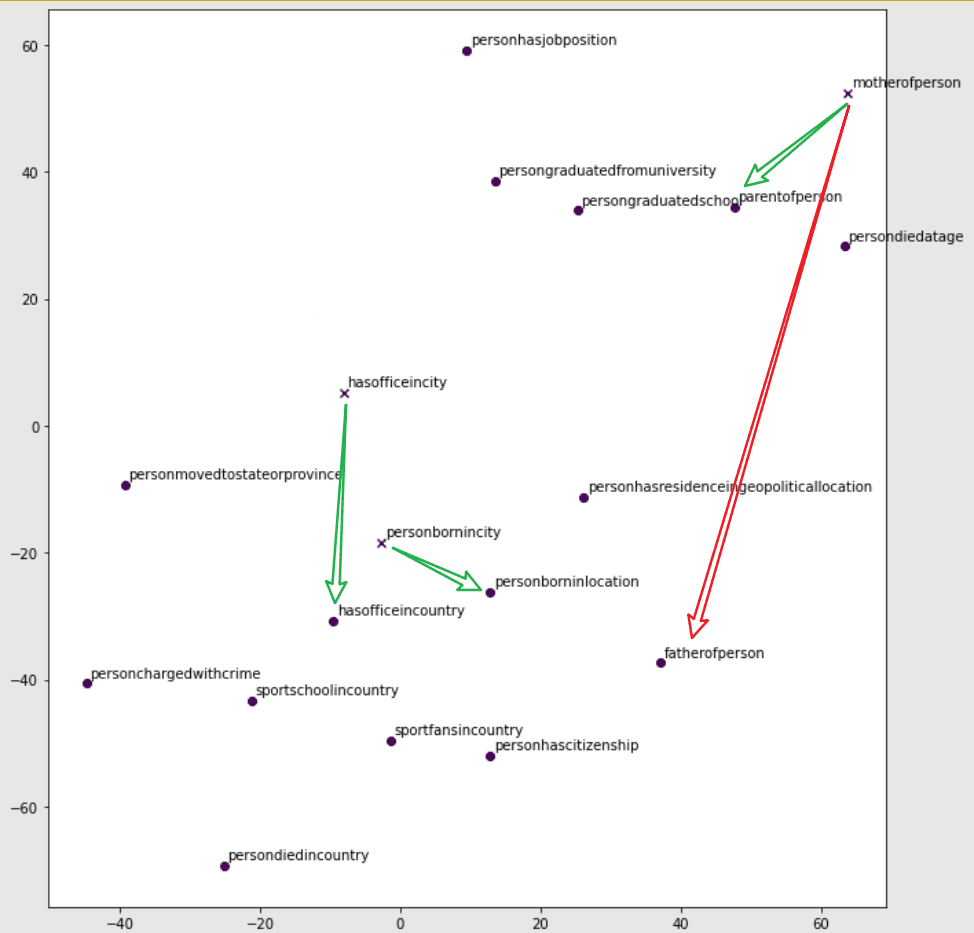
\includegraphics[width=0.7\textwidth]{4-2.png}
  \caption{实体嵌入可视化分析}
  \label{fig:4-2}
\end{figure}

本文模型通过采用关系位置图、根据关系的相对位置对关系局部的邻接关系进行建模学习到了关系的拓扑结构信息,同时引入本体信息作为语义补充,因此同一实体的具有相近语义的相邻关系在距离上应该表现为更加相近,从图上可以看出,对于未见关系has\_office\_in\_city贴近于具有类似语义的关系has\_office\_in\_coutry,未见关系person\_born\_in\_city更贴近于已知关系person\_born\_in\_location。而对于已知关系parent\_of\_person、father\_of\_person和未见关系mother\_of\_person,本文可知一个实体如果存在parent\_of\_person的关系那么该实体节点的邻接关系中只能存在其中一个father或者mother的关系,因此在图中本文可以观察到mother\_of\_person在距离上更接近于parent\_of\_person关系,而远离father\_of\_person关系。由此可见,本文模型通过在关系的位置图上联合本体语义信息有效的学习到了对应关系的语义关系,且其中相似的关系在向量空间中靠近,证明了本文提出的NAMER在嵌入未知关系方面的有效性。

\section{本章小结}
本章将本文提出的模型在测试数据集上NELL\_Ext和DB\_Ext上进行了链接预测任务的相关实验。与多个基准模型相比,本文提出的模型在任务得分上均有不同程度的提升,并通过对实验结果的分析验证了模型对于表示学习效果增强的有效性。同时通过对各个模型组件的消融实验发现明显的效果下降,证明了模型模块的重要性;最后对未见实体和未见关系的案例分析可知得到的嵌入表示符合模型原理设定,再次证明了该模型对未见组件表示上的突出能力。